\documentclass[t]{beamer}
\usetheme{hkl}

\title{Correlation}
	\author{François Briatte \& Ivaylo Petev}
	\date{Week~\#7}

\begin{document}
	
    \frame[plain]{
		\titlepage\\[7em]
		\tableofcontents[hideallsubsections]
		}

	% http://www.kenbenoit.net/courses/iqrm/IQRM_Week7_Comparing.pdf
	% http://personalpages.manchester.ac.uk/staff/mark.lunt/stats/4_Hypothesis_testing_and_power/practical.pdf
	% http://gabrielr.bol.ucla.edu/soc210a_f09/w6.pdf
	% http://gabrielr.bol.ucla.edu/soc210a_f09/w7.pdf
	% http://faculty.washington.edu/cadolph/321/321lec8.pdf
	%
	%

	\section{Review: Statistical tests}
	
	\begin{frame}[c]{\thesection. Statistical tests}
		
		\vfill
		 
		\begin{columns}[T]
			\column{.2\textwidth}
			
			\includegraphics[height=.5\textheight]{ziliak-mccloskey}

			\column{.6\textwidth}
			
			\footnotesize{%
			\textbf{Additional references}\\[1em]%
			%
			Leahey, ``\href{http://sf.oxfordjournals.org/content/84/1/1}{Alphas and Asterisks: The Development of Statistical Significance Testing Standards in Sociology}'', \emph{Social Forces}, 2005.\\[1em]%
			%
			Ziliak and McCloskey, \emph{\href{http://www.press.umich.edu/titleDetailDesc.do?id=186351}{The Cult of Statistical Significance: How the Standard Error Costs Us Jobs, Justice, and Lives}}, University of Michigan Press, 2008.%
			}
		\end{columns}
	\end{frame}
	
	%
	%
	
	\begin{frame}{Hypothesis testing}
		 
		\begin{block}{Substantive hypotheses}
			There is an association between $X$ and $Y$, ...
			
			There is a difference of $X$ between groups of $Y$, ...
		\end{block}
		
		\begin{block}{Null hypothesis tests}
			$H_0$: the association of $X$ by $Y$ is likely to be random.

			$H_0$: the difference in $X$ between groups of $Y$ is likely to be random.
		\end{block}
		
		\begin{alertblock}{Rejecting the null}
			$H_0$ estimates the likelihood of an association or difference being attributable to \red{sampling error} under a certain \red{level of confidence}.
		\end{alertblock}
		
	\end{frame}

	%
	%

	\begin{frame}[c]{Hypothesis testing}
		
		\begin{columns}[c]
			\column{.5\textwidth}
			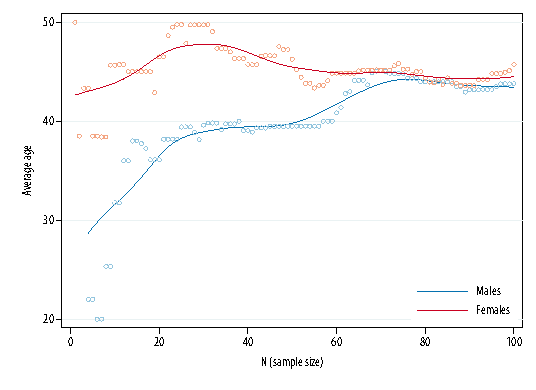
\includegraphics[width=\textwidth]{diff-age}
			
			\begin{center}
				Type I error
			\end{center}

			\column{.5\textwidth}
			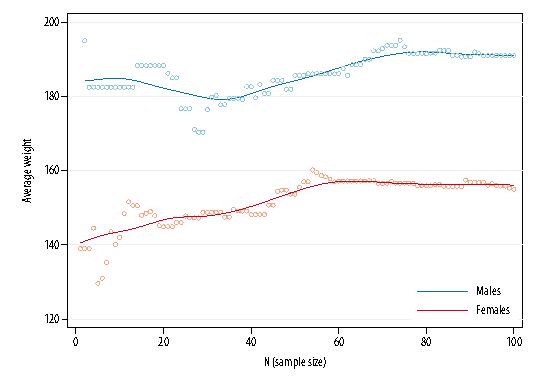
\includegraphics[width=\textwidth]{diff-weight}

			\begin{center}
				Type II error
			\end{center}
		\end{columns}
		
	\end{frame}

	%
	%

	\section{Review: $t$-test}

	%
	%
	
	\begin{frame}[c]{\thesection. $t$-test}

		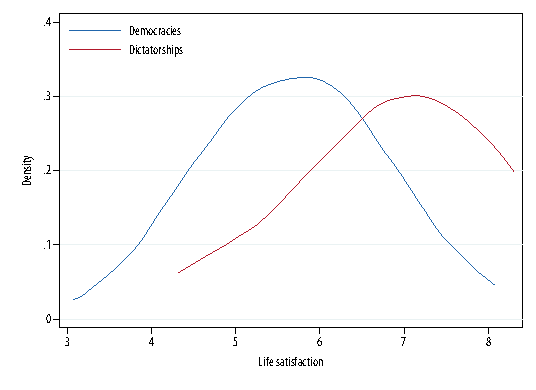
\includegraphics[width=\textwidth]{two-groups}

	\end{frame}
		
	\begin{frame}{$t$-test}
		
		\begin{block}{Measuring association as the difference in means between two groups of i.i.d.~observations:}
		
			\begin{itemize}
				\item Population notation:
				$\delta = \mu_1 - \mu_2$

				\item Sample notation:
				$D = \bar X_1 - \bar X_2$
			\end{itemize}

		\end{block}
		
		\begin{block}{The $t$-test computes a 95\% CI around the difference of their means and returns its $p$-value against the $t$-distribution.}
		
			\begin{itemize}
				\item Null hypothesis $H_0$:
				$\mu_1 - \mu_2 = 0$
			
				\item Test statistic:
				$t = \frac{D}{SE_D}$
			\end{itemize}

		\end{block}
		
	\end{frame}

	%
	%

	\begin{frame}[t]{$t$-test}
		
		\begin{block}{\texttt{ttest v1, by(v2)}}

			\begin{itemize}
				\item \texttt{v1} is continuous, \texttt{v2} is a dummy
				\item use \texttt{prtest} if \texttt{v1} is also a dummy (proportions test)
				\item use \texttt{tab, gen()} to create dummies from categorical variables
			\end{itemize}

		\end{block}

        \begin{exampleblock}{\texttt{use datasets/qog2011, clear}}
			
			\begin{itemize}
				\item Variables: \texttt{d gol\_enep gol\_est2}
				\item Create dummies and compare parties across electoral systems.
			\end{itemize}
			
        \end{exampleblock}
	
	\end{frame}

	%
	%
	
	\begin{frame}[t]{$t$-test}

		% \begin{block}{\texttt{prtest v1, by(v2)}}
		% 
		% 	\begin{itemize}
		% 		\item \texttt{v1} and \texttt{v2} are both dummies (proportions) 
		% 		\item the rest of the test works (almost) like the $t$-test
		% 	\end{itemize}
		% 
		% \end{block}
		
		\begin{exampleblock}{\texttt{use datasets/qog2011, clear}}
			
			% \begin{itemize}
			% 	\item Run a proportions test: \texttt{prtest no\_mes, by(gol\_polreg)}
			Explore the variables and interpret the output below.
			% \end{itemize}
						
        \end{exampleblock}

		\begin{center}
			\includegraphics[width=.8\textwidth]{prtest-mes}
		\end{center}
        
	\end{frame}

	%
	%
	
	\section{Review: Chi-squared test}
	
	%
	%
	
	\begin{frame}[c]{\thesection. Chi-squared test}

		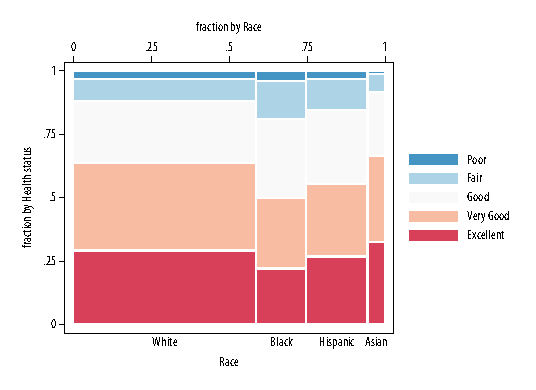
\includegraphics[width=\textwidth]{spineplot-health}
		
	\end{frame}
	
	%
	%

	% \begin{frame}[c]{\texttt{spineplot}}
	% 
	% 	\includegraphics[width=\textwidth]{spineplot-marstat}
	% 			
	% \end{frame}
	
	%
	%

	\begin{frame}{Chi-squared test}
		
		\begin{block}{The Chi-squared test is a nonparametric test of association that measures the deviation in orthogonality between groups:}
		
			\begin{itemize}
				\item Null hypothesis $H_0$:
				$\chi^2=0$
			
				\item Test statistic:
				%
				$\chi^2=\sum_{i=1}^{n} \frac{(O_i - E_i)^2}{E_i}$ (deviation between observed frequencies $O_i$ and expected frequencies $E_i$ for each table cell $i$)
				
			\end{itemize}

		\end{block}
		
		\begin{block}{\texttt{tab v1 v2, \red{exp chi2 V}}}

			\begin{itemize}
				\item add \texttt{V} to measure the association with Cramér's $V$ ($0 < V < 1$)
				\item use \texttt{tabchi} to inspect residuals, \texttt{tabodds} for odds ratios
			\end{itemize}

		\end{block}
		
	\end{frame}
	
	%
	%
	
	\begin{frame}[t]{Chi-squared test}
		
		\begin{exampleblock}{use datasets/nhis2009, clear}
		
			\begin{itemize}
				\item Variables: \texttt{d raceb marstat}
							
				\item Analyze the frequencies and residuals with \texttt{tabchi}
				
			\end{itemize}

		\end{exampleblock}
		
		\begin{center}
			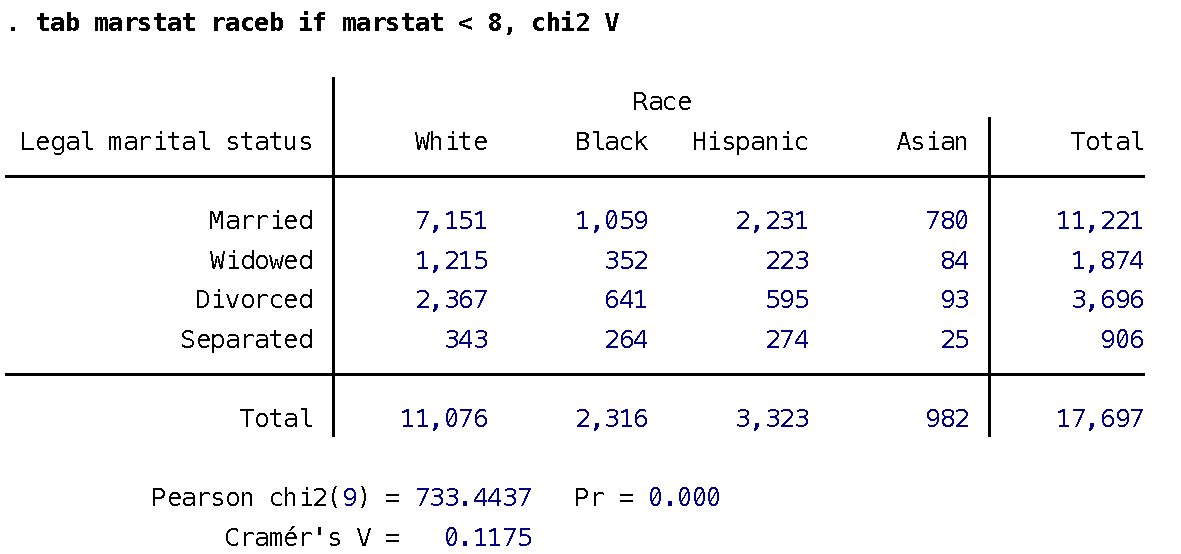
\includegraphics[width=.8\textwidth]{chi2-marstat}
		\end{center}
		
	\end{frame}
		
	%
	%
	
	\section{Correlation}
	
    \begin{frame}[c]{\thesection.~Correlation}
	
		\begin{center}
			\includegraphics[height=6.5cm]{corr-sc}
		\end{center}
				
	\end{frame}
	
	\begin{frame}{Pearson correlation coefficient}
	
		\begin{block}{Measuring association as the linear dependence of two variables:}
		
			\begin{align*}
				\text{Population notation} \quad
				\rho &= \frac{\text{Cov}(X,Y)}{\text{Var}_X\text{Var}_Y}, \quad
				-1 \leq \rho \leq 1
				\\
				\text{Sample notation} \quad
				r &= \frac{1}{n-1} \sum ^n _{i=1} (\frac{X_i - \bar{X}}{s_X}) (\frac{Y_i - \bar{Y}}{s_Y})
			\end{align*}

		\end{block}
		
		\begin{alertblock}{Detects linear correlation}

			\begin{itemize}
				\item Uncorrelated $\neq$ unrelated
				\item Correlated $\neq$ unconfounded
			\end{itemize}
						
		\end{alertblock}
					
	\end{frame}

	%
	%

	\begin{frame}[c]{Perfect (positive, negative) correlation}
			
		\begin{center}
			\includegraphics[width=\textwidth]{corr1}		
		\end{center}

	\end{frame}	

	\begin{frame}[c]{Significant (moderate, strong) correlation}
			
		\begin{center}
			\includegraphics[width=\textwidth]{corr2}		
		\end{center}

	\end{frame}	

	\begin{frame}[c]{Insignificant (weak, non-linear) correlation}
			
		\begin{center}
			\includegraphics[width=\textwidth]{corr3}		
		\end{center}

	\end{frame}
	
	%
	%
	
	\begin{frame}{Pearson correlation coefficient}
	
		\begin{block}{Significance test:}

			\begin{align*}
				\text{Null hypothesis~} H_0 \quad
				r &= 0
				\\
				\text{Test statistic} \quad
				T &= r \sqrt{\frac{n-2}{1-r^2}}
			\end{align*}

		\end{block}
		
		\begin{alertblock}{Sanity check}

			\begin{itemize}
				\item Uncorrelated $\neq$ independent
				\item Correlated $\neq$ causally related
			\end{itemize}
			
		\end{alertblock}
						
	\end{frame}
		
	%
	%
	
    \begin{frame}[c]

		\begin{center}
			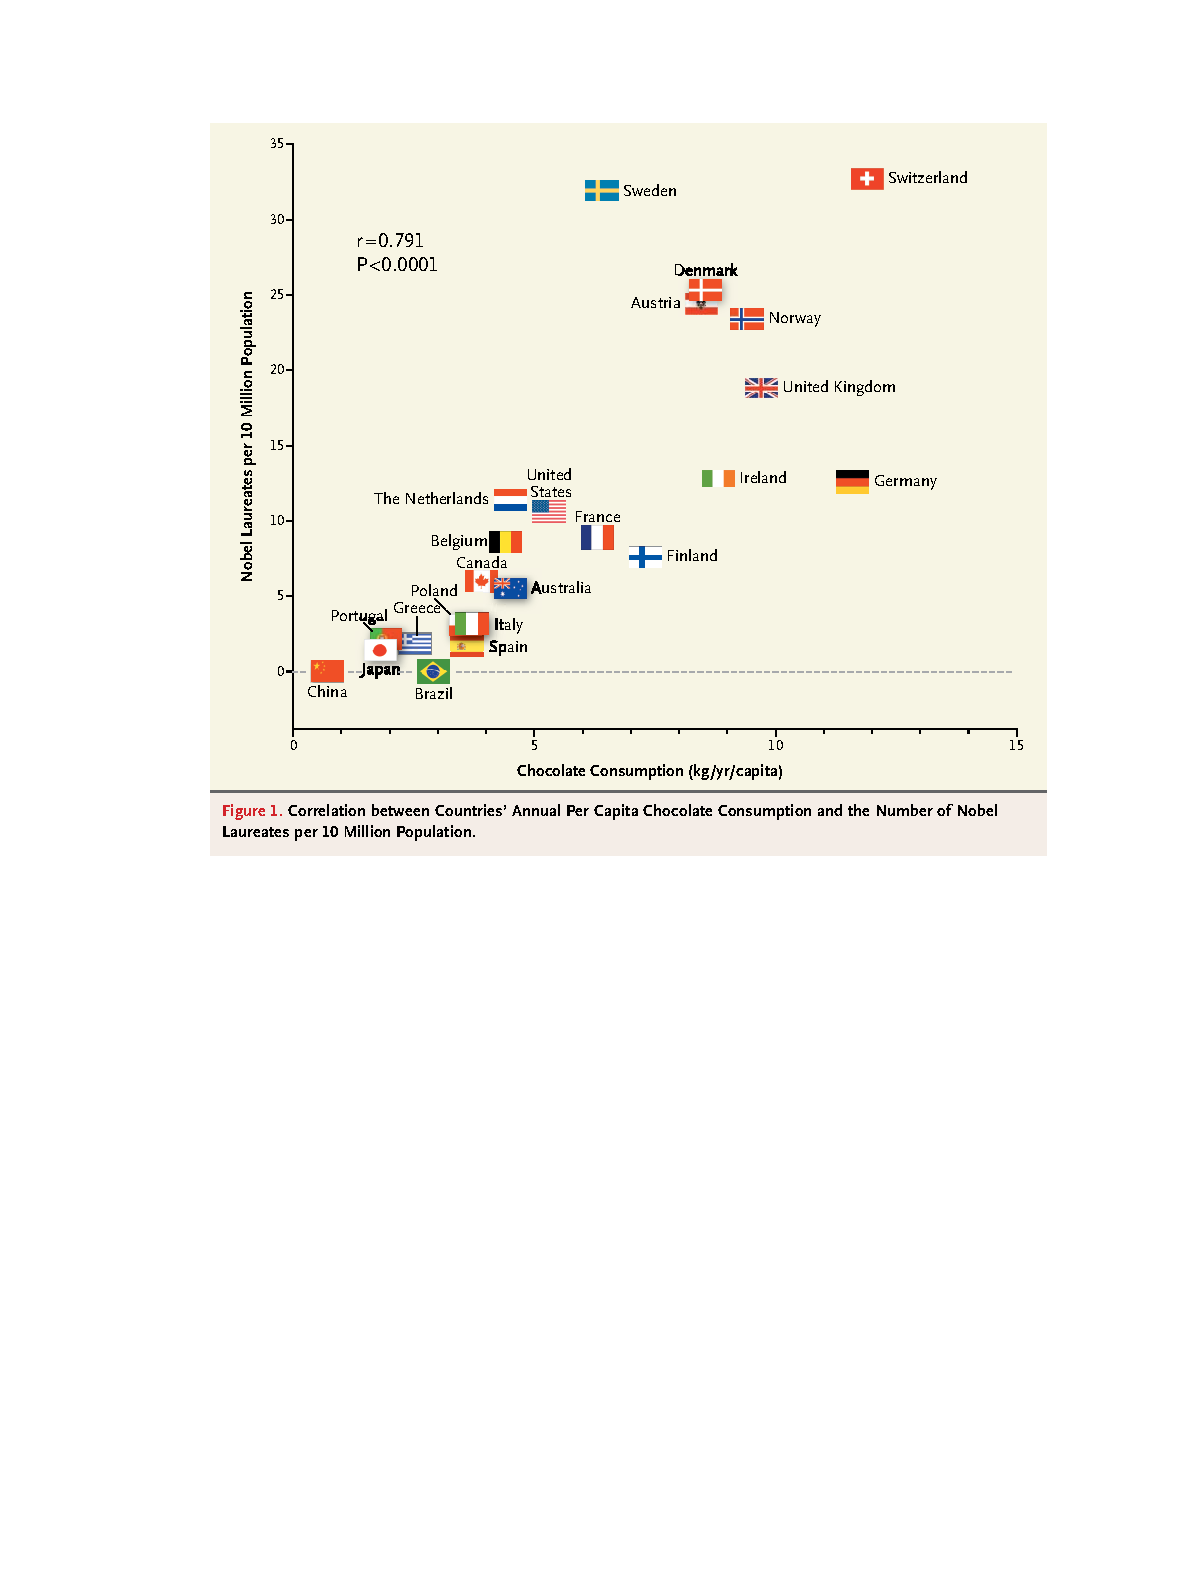
\includegraphics[height=6.5cm]{chocolate-nobel}
		\end{center}
		
		\vfill \par Source: Messerli, ``\href{http://www.nejm.org/doi/pdf/10.1056/NEJMon1211064}{Chocolate Consumption, Cognitive Function, and Nobel Laureates}'', \emph{New England Journal of Medicine}, 2012.
		
	\end{frame}

	%
	%
	
	\begin{frame}[c]

		\begin{center}
			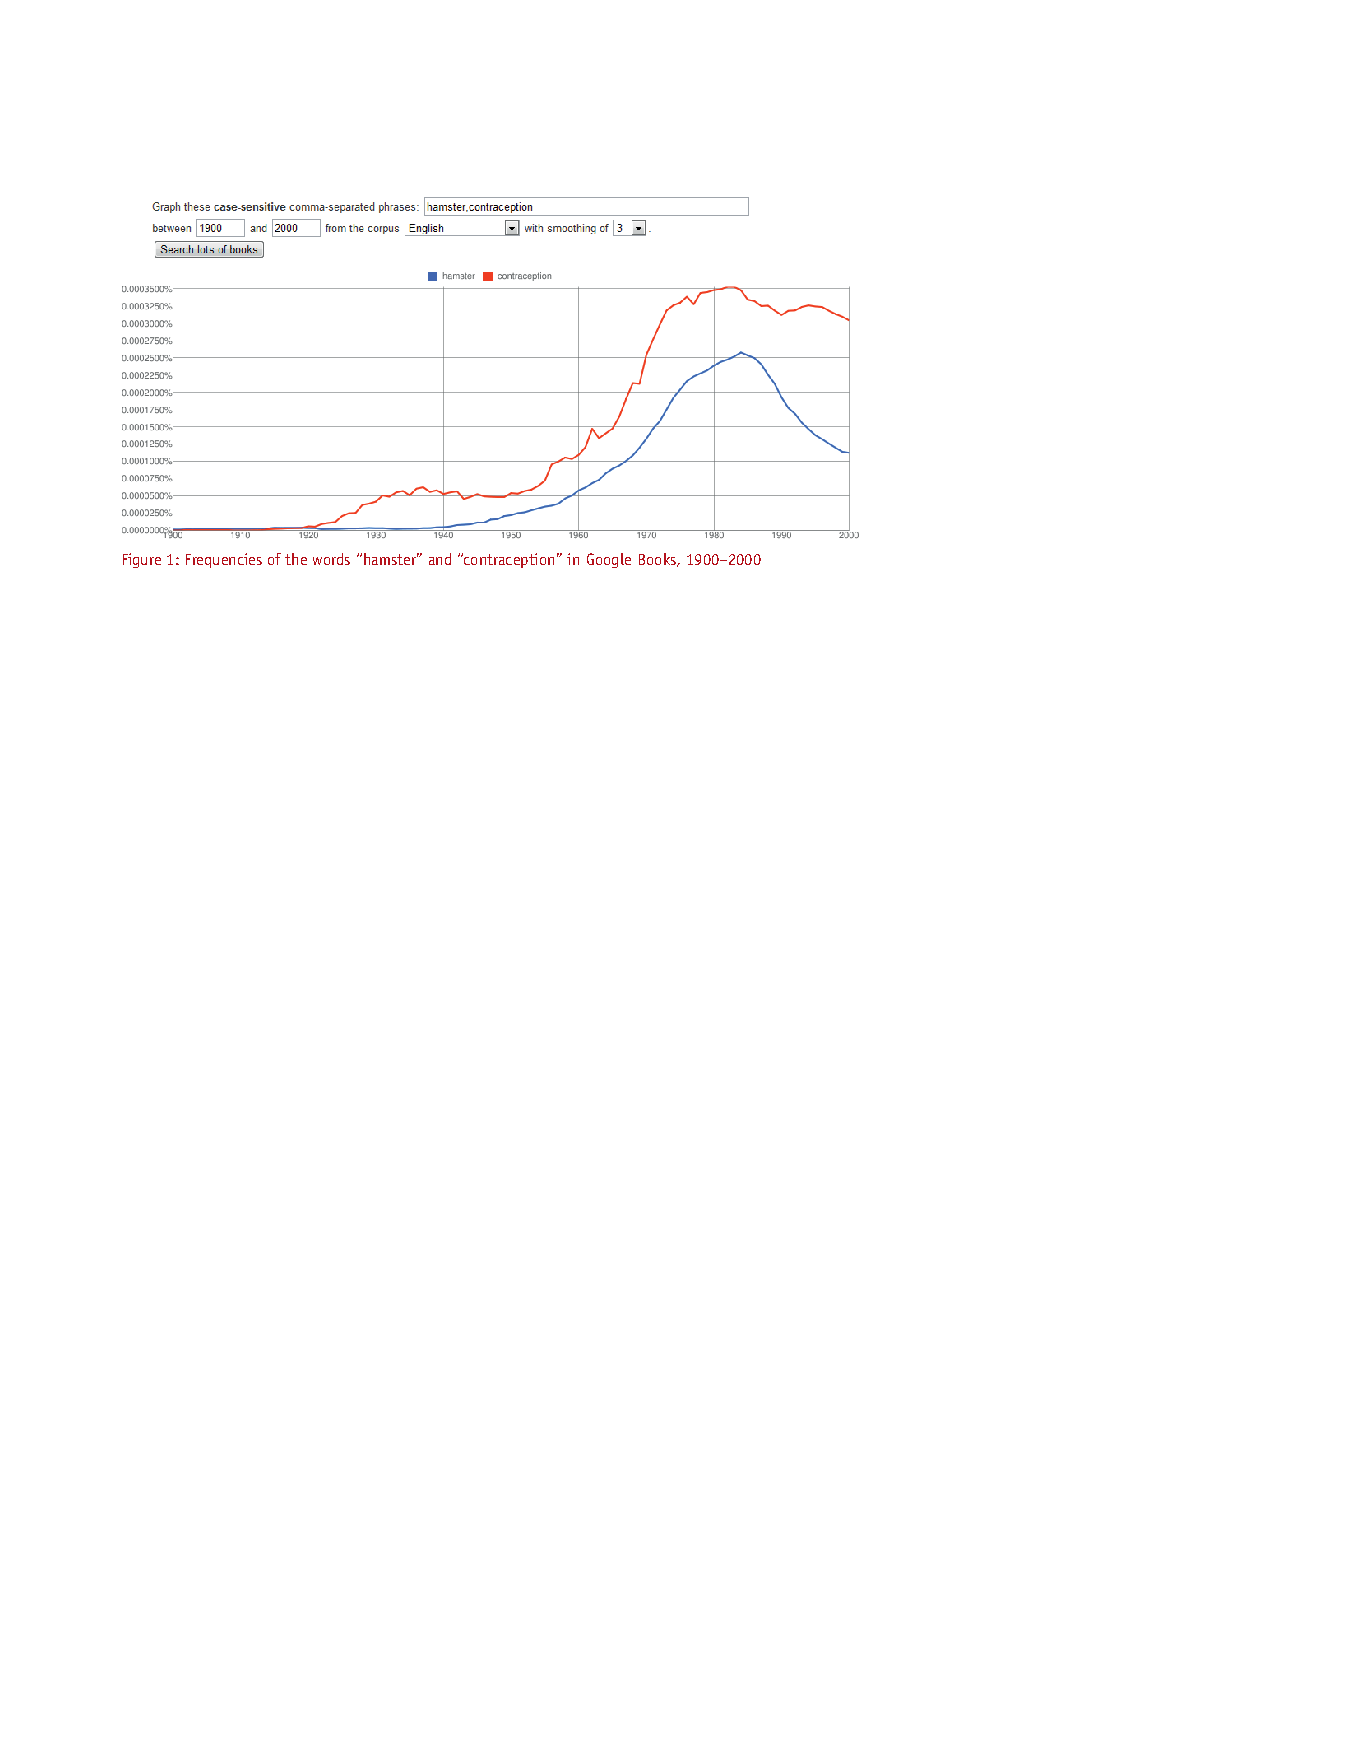
\includegraphics[width=\textwidth]{hamster-contraception}	
		\end{center}
		
		\vfill \par Source: Harkness, ``\href{http://onlinelibrary.wiley.com/doi/10.1111/j.1740-9713.2012.00549.x/abstract}{Seduced by Stats?}'', \emph{Significance}, 2012.
		
	\end{frame}

	%
	%

    \begin{frame}[c]{Correlation matrixes}
		
		\begin{block}{\texttt{pwcorr [varlist], [obs sig]}}

	        \begin{itemize}
	          \item \texttt{obs} shows the number of observations
			  \item \texttt{sig} shows the coefficient's $p$-value
	        \end{itemize}

		\end{block}

		\begin{block}{\texttt{gr mat [varlist], [half etc.]}}		

	        \begin{itemize}
	          \item \texttt{half} plots only half of all graphs (quicker)
			  \item accepts scatterplot options (\texttt{jitter}, \texttt{mlab}, etc.)
	        \end{itemize}

		\end{block}
		
			%         \begin{exampleblock}{\texttt{use datasets/qog2011, clear}}
			% 
			% \begin{itemize}
			% 	\item Variables: \texttt{d wdi\_brd wdi\_mege wdi\_pb2 wdi\_the}
			% 	\item Inspect and plot the correlation matrix.
			% \end{itemize}
			% 
			%         \end{exampleblock}
	
	\end{frame}

	%
	%

    \begin{frame}[c]{Correlation matrixes}
	
		\begin{block}{\texttt{mkcorr [varlist], lab num sig log(file.txt) replace}}
			\begin{itemize}
				\item \texttt{ssc install mkcorr} to install
				\item \texttt{help mkcorr} to understand the options
			\end{itemize}
		\end{block}
	
		\begin{alertblock}{Computer skills}
			\begin{itemize}
				\item Import as a table in a spreadsheet editor.
				\item Convert from text to table in a rich text editor.
			\end{itemize}
			  
		\end{alertblock}

        \begin{exampleblock}{\texttt{use datasets/qog2011, clear}}
			
			\begin{itemize}
				\item Variables: \texttt{d wdi\_puhegdp wdi\_the wdi\_prhe}
				\item Visualize, compute, export and import the correlation matrix.
			\end{itemize}
			
        \end{exampleblock}

	\end{frame}
		
	%
	%

	% \begin{frame}[c]{One variable, many predictors}
	% 
	% 	\begin{center}
	% 		\includegraphics[width=.7\textwidth]{hate-sc1}	
	% 	\end{center}
	% 	
	% 	\par Source: Florida, ``\href{http://www.theatlantic.com/national/archive/2011/05/the-geography-of-hate/238708/}{The Geography of Hate}'', \emph{The Atlantic}, 2011.
	% 	
	% \end{frame}
	% 
	% \begin{frame}[c]{One variable, many predictors}
	% 
	% 	\begin{center}
	% 		\includegraphics[width=.7\textwidth]{hate-sc2}	
	% 	\end{center}
	% 	
	% 	\par Source: Florida, ``\href{http://www.theatlantic.com/national/archive/2011/05/the-geography-of-hate/238708/}{The Geography of Hate}'', \emph{The Atlantic}, 2011.
	% 	
	% \end{frame}
	% 
	% \begin{frame}[c]{One variable, many predictors}
	% 
	% 	\begin{center}
	% 		\includegraphics[width=.7\textwidth]{hate-sc3}	
	% 	\end{center}
	% 	
	% 	\par Source: Florida, ``\href{http://www.theatlantic.com/national/archive/2011/05/the-geography-of-hate/238708/}{The Geography of Hate}'', \emph{The Atlantic}, 2011.
	% 	
	% \end{frame}
	% 
	% \begin{frame}[c]{One variable, many predictors}
	% 
	% 	\begin{center}
	% 		\includegraphics[width=.7\textwidth]{hate-sc4}	
	% 	\end{center}
	% 	
	% 	\par Source: Florida, ``\href{http://www.theatlantic.com/national/archive/2011/05/the-geography-of-hate/238708/}{The Geography of Hate}'', \emph{The Atlantic}, 2011.
	% 	
	% \end{frame}
	% 
	% \begin{frame}[c]{One variable, many predictors}
	% 
	% 	\begin{center}
	% 		\includegraphics[width=.7\textwidth]{hate-sc5}	
	% 	\end{center}
	% 	
	% 	\par Source: Florida, ``\href{http://www.theatlantic.com/national/archive/2011/05/the-geography-of-hate/238708/}{The Geography of Hate}'', \emph{The Atlantic}, 2011.
	% 	
	% \end{frame}

	%
	%

	\begin{frame}[c]{\texttt{gr mat}}

		\includegraphics[width=\textwidth]{gr-mat}
				
	\end{frame}
	
	\begin{frame}[t]{From Stata output...}

		\begin{tikzpicture}
			\node[anchor=south west,inner sep=0] (image) at (0,0) {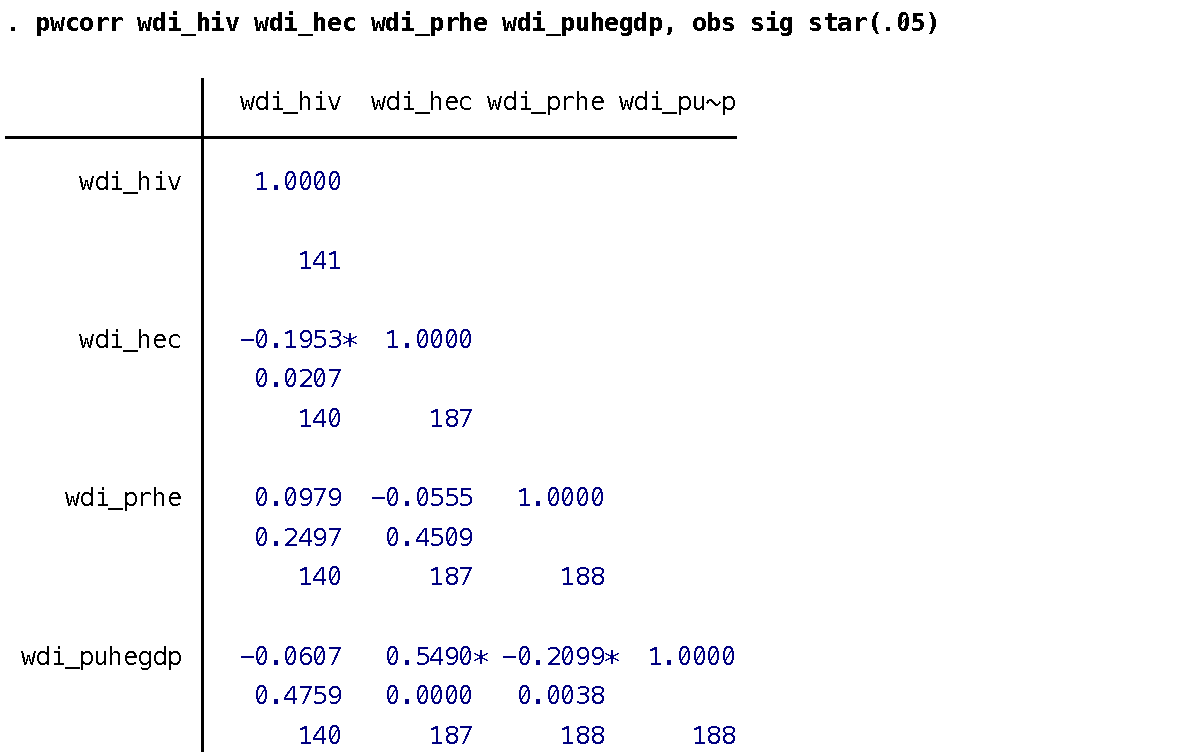
\includegraphics[width=.8\textwidth]{pwcorr}};
			
		    \begin{scope}[x={(image.south east)},y={(image.north west)}]
				\draw[fill=blue, opacity=0.25] (.32, .11) rectangle (.42, .17);
				\draw[fill=red, opacity=0.25] (.43, .05) rectangle (.53, .11);
				\draw[fill=green, opacity=0.25] (.54, -.01) rectangle (.64, .05);
		    		\node[anchor=west, fill=blue, text opacity=1, opacity=0.25] at (.8, .22) { coefficient };
		    		\node[anchor=west, fill=red, text opacity=1, opacity=0.25] at (.8, .10) { $p$-value };
		    		\node[anchor=west, fill=green, text opacity=1, opacity=0.25] at (.8, -.02) { observations };
%				\draw[help lines,xstep=.1,ystep=.1] (0,0) grid (1,1);
%				\foreach \x in {0,1,...,9} { \node [anchor=north] at (\x/10,0) {0.\x}; }
%				\foreach \y in {0,1,...,9} { \node [anchor=east] at (0,\y/10) {0.\y}; }
				\draw[fill=yellow, opacity=0.25] (.19, .42) rectangle (.31, .58);
		    		\node[anchor=west, fill=yellow, text opacity=1, align=left, opacity=0.25] at (.8, .58) { $r = -.2$ \\ $p < .02$ \\ $N = 140$ };
		    \end{scope}
		\end{tikzpicture}
			
	\end{frame}

	\begin{frame}[t]{... to publishing standard}

		\begin{center}
			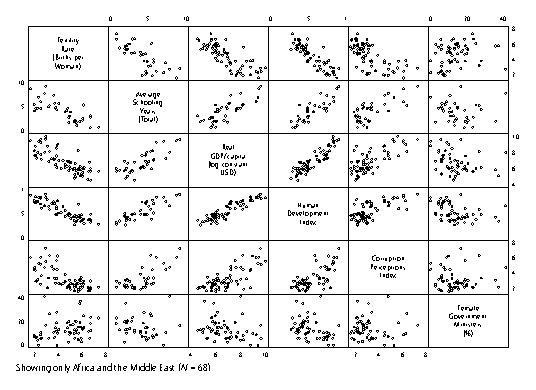
\includegraphics[width=\textwidth]{correlation-matrix}	
		\end{center}
		
		\vfill \par Source: Adhikari \emph{et al.}, ``Public Policy, Political Connections, and Effective Tax Rates: Longitudinal Evidence from Malaysia'', \emph{Journal of Accounting and Public Policy}, 2006.
		
	\end{frame}
	
	%
	%

	\subsection{Coursework}

	\begin{frame}[c]{Coursework}

		\begin{alertblock}{Project}
			\begin{itemize}
				\item Start testing associations in your data
				\item Refine hypotheses and write draft findings
			\end{itemize}
		\end{alertblock}
		
		\begin{block}{Readings}
			\begin{itemize}
				\item \emph{Stata Guide}, Sec.~10 (association)
				\item \emph{Making History Count}, ch.~3 (correlation)
			\end{itemize}
		\end{block}
			
		\begin{exampleblock}{Practice}
			\begin{itemize}
				\item Replicate do-file
				\item Exercises in slides
			\end{itemize}
		\end{exampleblock}
			
	\end{frame}
	
\end{document}
